\begin{scanpage}{0053}{36}
\begin{center}\begin{minipage}[t]{.48\linewidth}\vspace{0pt}\centering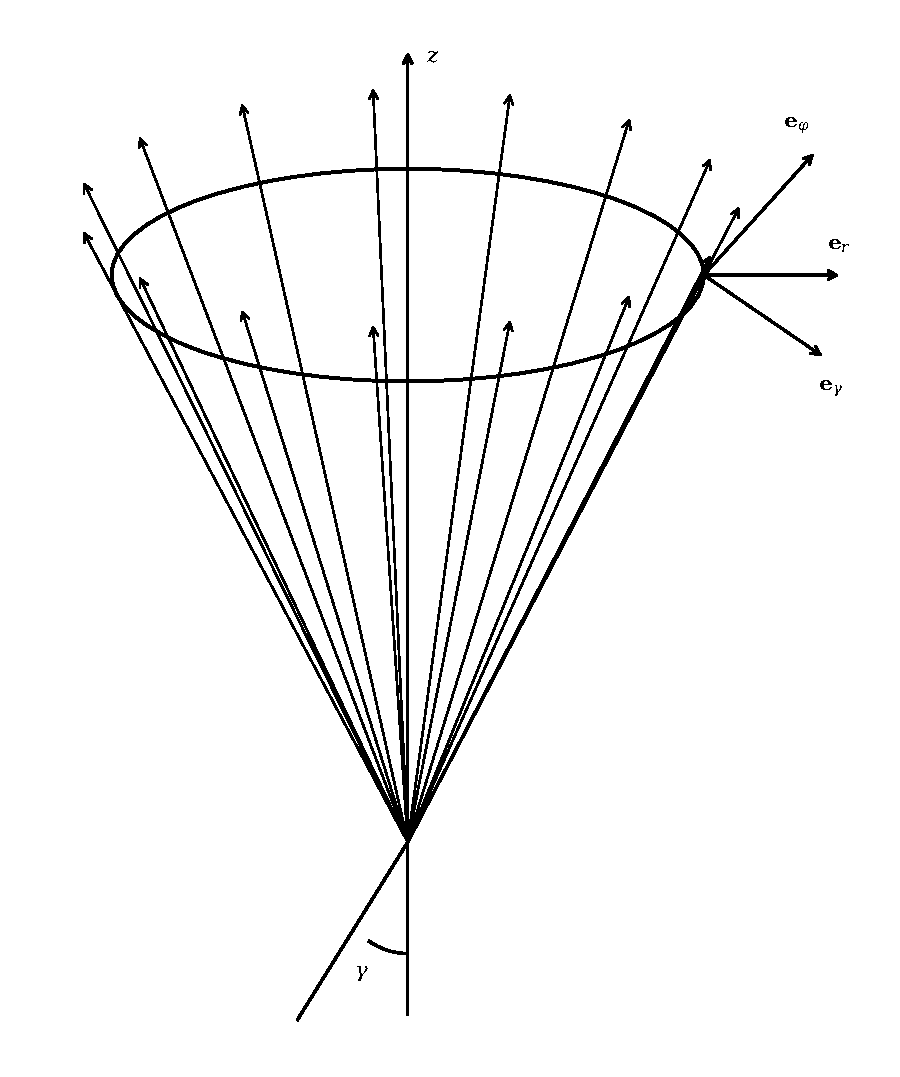
\includegraphics[height=4.5cm]{images/recreated/a-0053-fig15.pdf}\par Figure 15. The cone of diffracted rays.\end{minipage}\hfill\begin{minipage}[t]{.48\linewidth}\vspace{0pt}\centering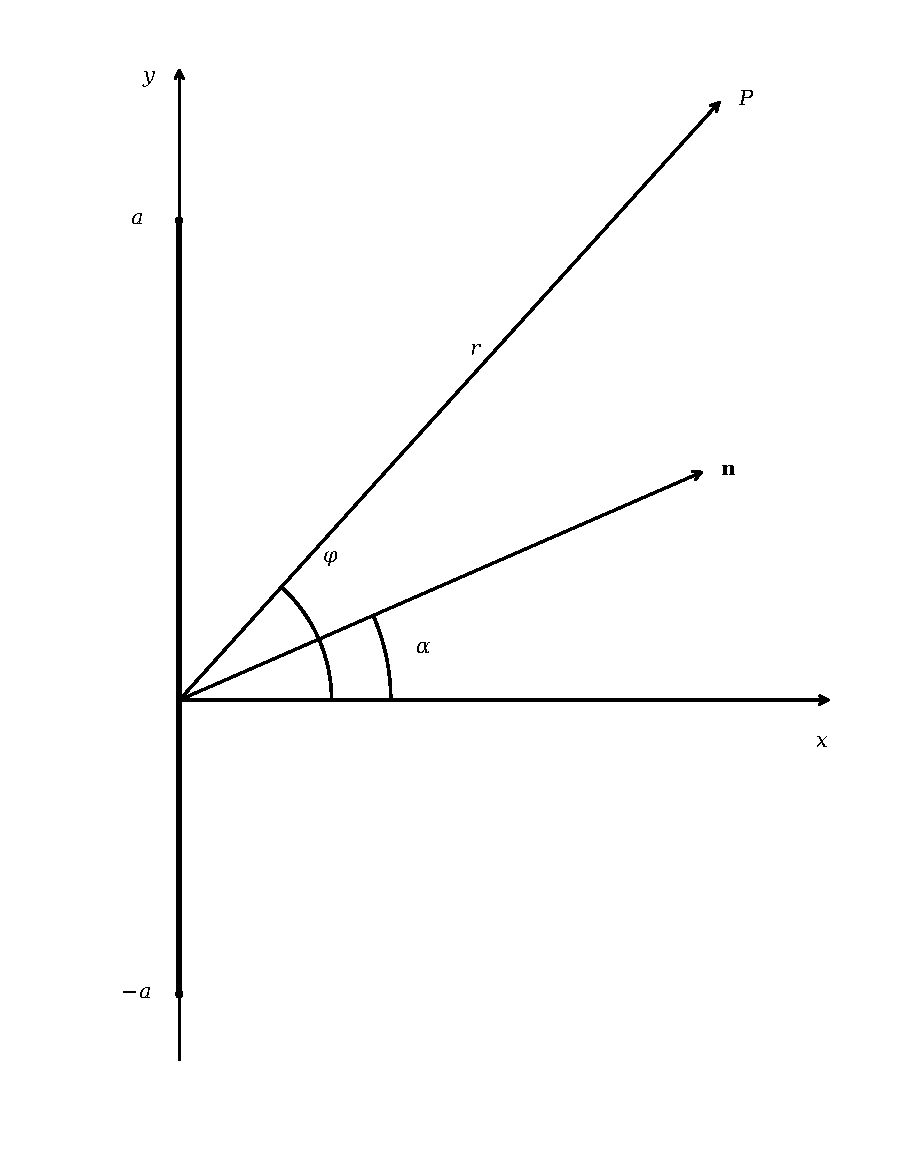
\includegraphics[height=4cm]{images/recreated/a-0053-fig16.pdf}\par Figure 16. Diffraction of a plane wave by an infinitely long strip. The section of the axis $y$ $(-a\leq y\leq a)$ shows the transverse cross section of the strip with the plane $z=0$; $\alpha$ is the angle of incidence.\end{minipage}\end{center}
Let a plane, electromagnetic wave strike the strip perpendicular to the edges. Let the direction of propagation of this wave form an angle $\alpha$ $\left(|\alpha|<\frac\pi2\right)$ with the plane $y=0$. The field of this wave is represented in the form
\[\mathbf E=\mathbf E_0e^{ik(x\cos\alpha+y\sin\alpha)},\quad\mathbf H=\mathbf H_0e^{ik(x\cos\alpha+y\sin\alpha)}.\tag{6.01}\]
The uniform part of the current excited by the plane wave on the strip has the components
\[\left.\begin{aligned}j_x^0&=0,\\j_y^0&=\frac c{2\pi}H_{0z}e^{iky\sin\alpha},\\j_z^0&=\frac c{2\pi}E_{0z}\cos\alpha\,e^{iky\sin\alpha}.\end{aligned}\right\}\tag{6.02}\]
Substituting these values into the equation for the vector potential
\end{scanpage}
